\section{Aufbau}
Der Aufbau des zylinderförmigen Germaniumdetektors ist in Abbildung \ref{fig:Aufbau} dargstellt. Wie dort zu sehen ist, besteht die Oberfläche des Detektors aus einer mit Lithium dotierten $n$-Schicht die als $+$-Pol dient. Im inneren des Detektorkristalls befindet sich eine koaxiliale Bohrung. Deren innere Oberfläche wurde mit Gold bedampft und stellt somit eine $p$-dortierte Schicht da. Zwischen diesen Schichten befindet sich ein reiner Germaniumkristall, in dem sich aufgrund der $p$ - und $n$-dotierten Schichten zur Ausbildung einer ausgedehnten Verarmungszone kommt. 
\begin{figure}[H]
    \centering
    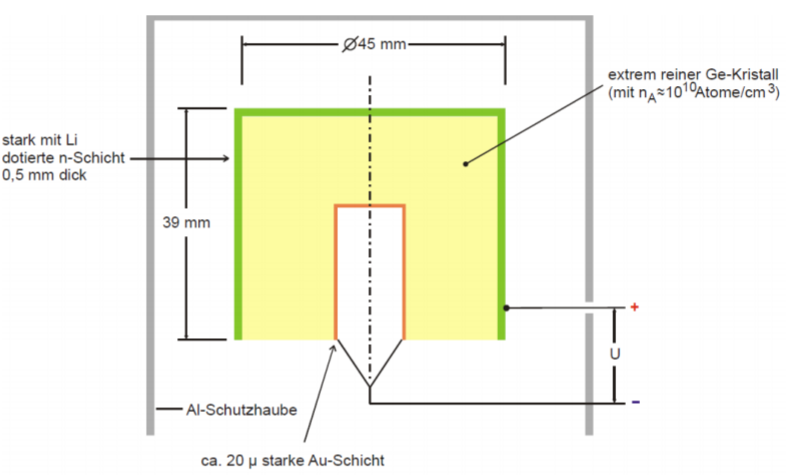
\includegraphics[width=0.8\textwidth]{content/images/Aufbau.png}
    \caption{Koaxialquerschnitt des Detektors \cite{anleitung} }
    \label{fig:Aufbau}
\end{figure}
Einfallende Photonen müssen zuerst die Aluminium-Schutzhaube durchqueren, die den Detektor umgibt, bevor an die $n$-dotierte Schichte gelangen. Daher existiert eine untere Nachweisgrenze von $40-50 \si{\kilo \electronvolt}$ sowie eine Vollenergienachweisgrenze von ca. $150 \si{\kilo \electronvolt}$ für Photonen.

\section{Durchführung}
Zunächst wird ein $^{152}\symup{Eu}$-Strahler mit bekannter Aktivität dazu verwendet, den Detektor zu kalibrieren und die Vollenergienachweiswahrscheinlichkeit zu bestimmen. Anschließend werden die Aktivitäten von $^{137}\symup{Cs}$- und  $ ^{133}\symup{Ba} $ Proben mit dem Detektor untersucht. Zum Schluss wird die Aktivität einer unbekannten Probe untersucht, um auf die Probe zurückzuschließen. 